\documentclass[a4paper,12pt]{article}
%%% Работа с русским языком
\usepackage[unicode, pdftex]{hyperref}
\usepackage{cmap}					% поиск в PDF
\usepackage{mathtext} 				% русские буквы в формулах
\usepackage[T2A]{fontenc}			% кодировка
\usepackage[utf8]{inputenc}			% кодировка исходного текста
\usepackage[english,russian]{babel}	% локализация и переносы
\usepackage{indentfirst}
\frenchspacing


\renewcommand{\epsilon}{\ensuremath{\varepsilon}}
\renewcommand{\phi}{\ensuremath{\varphi}}
\renewcommand{\kappa}{\ensuremath{\varkappa}}
\renewcommand{\le}{\ensuremath{\leqslant}}
\renewcommand{\leq}{\ensuremath{\leqslant}}
\renewcommand{\ge}{\ensuremath{\geqslant}}
\renewcommand{\geq}{\ensuremath{\geqslant}}
\renewcommand{\emptyset}{\varnothing}

%%% Дополнительная работа с математикой
\usepackage{amsmath,amsfonts,amssymb,amsthm,mathtools} % AMS
\usepackage{icomma} % "Умная" запятая: $0,2$ --- число, $0, 2$ --- перечисление

%% Номера формул
%\mathtoolsset{showonlyrefs=true} % Показывать номера только у тех формул, на которые есть \eqref{} в тексте.
%\usepackage{leqno} % Нумереация формул слева

%% Свои команды
\DeclareMathOperator{\sgn}{\mathop{sgn}}

%% Перенос знаков в формулах (по Львовскому)
\newcommand*{\hm}[1]{#1\nobreak\discretionary{}
	{\hbox{$\mathsurround=0pt #1$}}{}}

%%% Работа с картинками
\usepackage{graphicx}  % Для вставки рисунков
%\graphicspath{{images/}{images2/}}  % папки с картинками
\setlength\fboxsep{3pt} % Отступ рамки \fbox{} от рисунка
\setlength\fboxrule{1pt} % Толщина линий рамки \fbox{}
\usepackage{wrapfig} % Обтекание рисунков текстом

%%% Работа с таблицами
\usepackage{array,tabularx,tabulary,booktabs} % Дополнительная работа с таблицами
\usepackage{longtable}  % Длинные таблицы
\usepackage{multirow} % Слияние строк в таблице

%%% Теоремы
\theoremstyle{plain} % Это стиль по умолчанию, его можно не переопределять.
\newtheorem{theorem}{Теорема}[section]
\newtheorem{proposition}[theorem]{Утверждение}

\theoremstyle{definition} % "Определение"
\newtheorem{corollary}{Следствие}[theorem]
\newtheorem{problem}{Задача}[section]

\theoremstyle{remark} % "Примечание"
\newtheorem*{nonum}{Решение}

%%% Программирование
\usepackage{etoolbox} % логические операторы

%%% Страница
\usepackage{extsizes} % Возможность сделать 14-й шрифт
\usepackage{geometry} % Простой способ задавать поля
\geometry{top=25mm}
\geometry{bottom=35mm}
\geometry{left=35mm}
\geometry{right=20mm}
%


\usepackage{setspace} % Интерлиньяж (расстояние между строками)
%\onehalfspacing % Интерлиньяж 1.5
%\doublespacing % Интерлиньяж 2
%\singlespacing % Интерлиньяж 1

\usepackage{lastpage} % Узнать, сколько всего страниц в документе.




\usepackage[usenames,dvipsnames,svgnames,table,rgb]{xcolor}
\hypersetup{				% Гиперссылки
	unicode=true,           % русские буквы в раздела PDF
	pdftitle={Заголовок},   % Заголовок
	pdfauthor={Автор},      % Автор
	pdfsubject={Тема},      % Тема
	pdfcreator={Создатель}, % Создатель
	pdfproducer={Производитель}, % Производитель
	pdfkeywords={keyword1} {key2} {key3}, % Ключевые слова
	colorlinks=true,       	% false: ссылки в рамках; true: цветные ссылки
	linkcolor=red,          % внутренние ссылки
	citecolor=black,        % на библиографию
	filecolor=magenta,      % на файлы
	urlcolor=cyan           % на URL
}


%\usepackage[style=authoryear,maxcitenames=2,backend=biber,sorting=nty]{biblatex}

\usepackage{multicol} % Несколько колонок

\usepackage{tikz} % Работа с графикой
\usepackage{pgfplots}
\usepackage{pgfplotstable}
\usepackage{floatrow}
\DeclareFloatSeparators{mysep}{\hspace{3cm}}
\thisfloatsetup{floatrowsep=mysep}

\newcommand{\e}[1]{
	\cdot 10^{#1}	
}

\newcommand{\s}[0]{
	\;	
}

\newcommand{\picref}[1]{
	\text{рис(\ref{#1})}
}

\begin{document}
\begin{titlepage}
	\centering
	\vspace{5cm}
	{\scshape\LARGE Московский физико-технический институт \par}
	\vspace{5cm}
	{\huge\bfseries Лабораторная работа \par}
	\vspace{0.5cm}
	{\huge\bfseries <<Электронно оптический преобразователь>> \par}
	\vspace{1cm}
	{\scshape\Large по курсу <<Вакуумная электроника>>\par}
	\vspace{1cm}
	\vfill
	
\begin{flushright}
	{\large выполнили студенты 004-007 групп ФФКЭ}\par
	\vspace{0.3cm}
	{\LARGE Голощапов Михаил, Атласов Владислав, Шарапов Алексей, Петрова София, Богатова Екатерина, Спирандэ Екатерина.} \par
\end{flushright}

	\vfill
% Bottom of the page
	Долгопрудный, 2022 г.
\end{titlepage}

	\newpage
	\section{Цель работы}
	
	\section{Теоретические сведения. Экспериментальная установка.}
	Электронно-оптические преобразователи (ЭОП) – это вакуумные приборы, сначала преобразующие оптическое изображение в электронный аналог, т.е. в электронное изображение, которым можно эффективно управлять электрическим полем (усиливать, отклонять по координате и т.д.), после чего оно проецируется на люминесцентный экран, где снова преобразуется в оптическое изображение. \\
	
ЭОП представляет собой электровакуумную колбу, внутри которой размещены фотокатод, люминесцентный экран,  фокусирующая и ускоряющая электронно-оптические системы. В ЭОП, используемом в лабораторной работе для усиления электрического тока применяется микроканальная пластина.
Когда налетающий электрон попадает в канал, то из стенки канала выбиваются вторичные электроны, которые ускоряются электрическим полем вдоль канала. Электрическое поле внутри канала создаётся путём приложения напряжения между поверхностями МКП (концами каналов). Вторичные электроны летят, пока не попадут на стенку, в свою очередь выбивая ещё большее количество вторичных электронов. Этот процесс по мере пролёта вдоль канала повторяется много раз, и на выходе канала формируется электронная лавина.\\

\begin{figure}[h]
\begin{center}
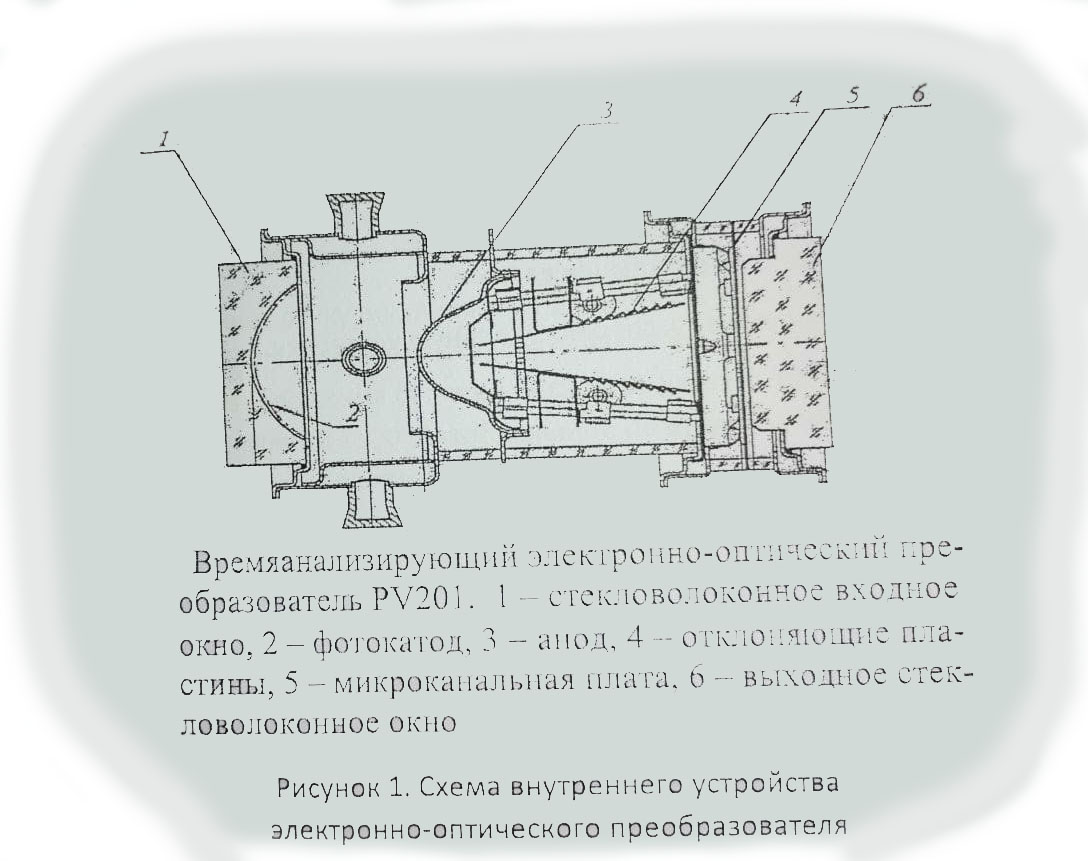
\includegraphics[width=0.7\linewidth]{схема устройства эоп.jpg}
\end{center}
\end{figure}

\begin{figure}[h]
\begin{center}
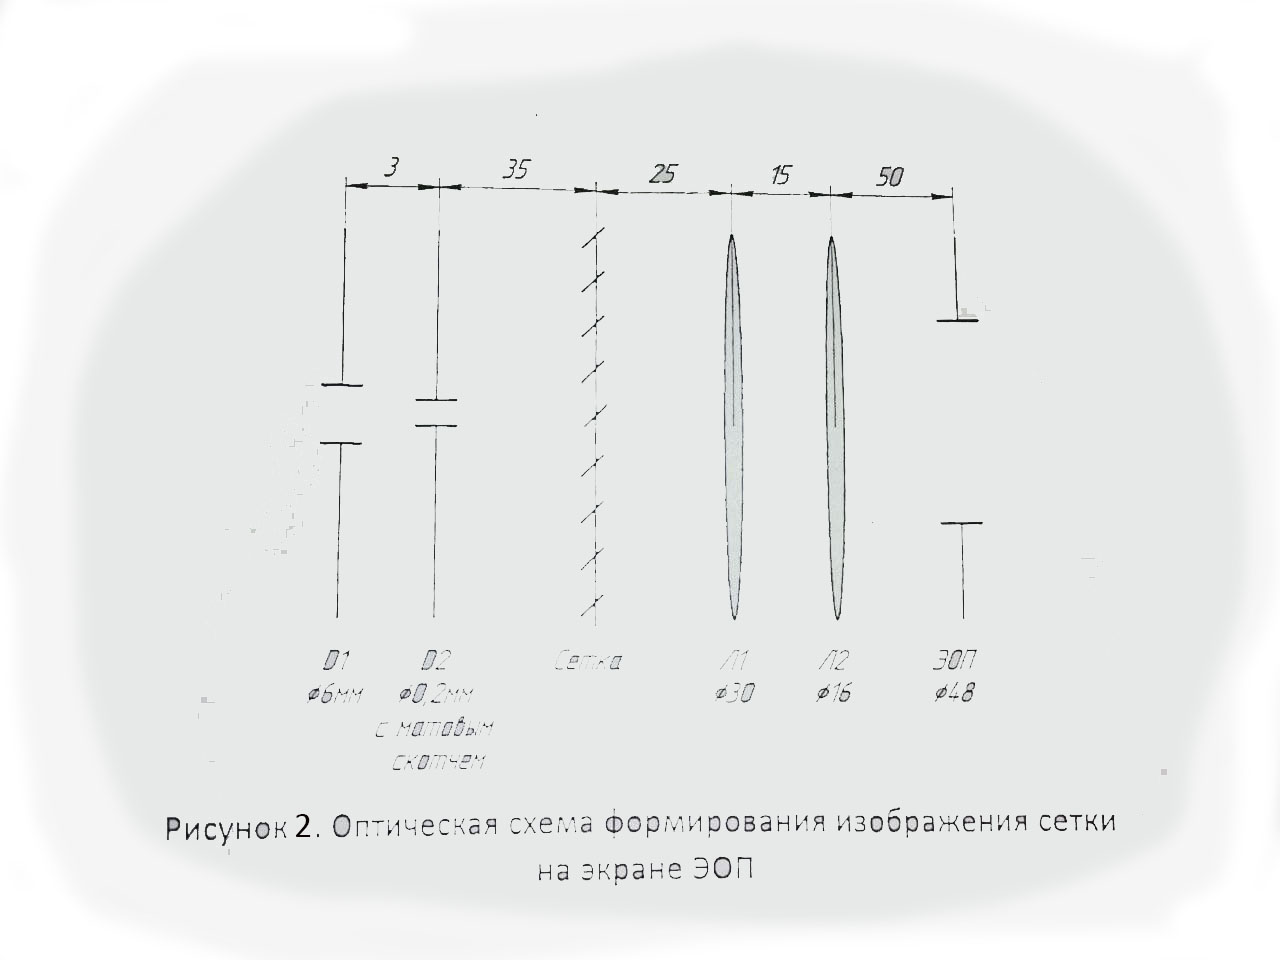
\includegraphics[width=0.7\linewidth]{опт схема эоп.jpg}
\end{center}
\end{figure}

\newpage

	\section{Ход работы и результаты измерений.}
\begin{enumerate}
    \item Приводим установку в рабочее состояние. При помощи ручек можно регулировать напряжение катода, напряжение экрана и напряжение МКП; регистрировать ток анода, катода, МКП и экрана. По умолчанию значения напряжений МКП, экрана и катода равны 1.2 кВ, 3.5 кВ и 3.5 кВ соответственно.
    \item При значениях напряжения на экране и МКП по умолчанию меняем напряжение на катоде от 0.9 кВ до 4.2 кВ и фиксируем значения всех токов (см. графики 1, 2, 3 и 4)
    \item  При значениях напряжения на экране и катоде по умолчанию меняем напряжение на МКП от 0.4 кВ до 1.8 кВ и фиксируем значения всех токов (см. графики 5, 6, 7 и 8)
    \item При значениях напряжения на катоде и МКП по умолчанию меняем напряжение на экране от 0.8 кВ до 3.5 кВ и фиксируем значения всех токов (см. графики 9, 10, 11 и 12)
    \item При максимальном напряжении на МКП понижаем напряжение на катоде до минимального уровня, при котором видно изображение. Далее мы понижаем напряжение на  МКП попутно повышая напряжение на катоде, стараясь сохранять постоянный уровень яркости изображения. Фиксируем значения напряжений (см. график 13)
    \item Понижаем все напряжения до нуля и отключаем установку.
\end{enumerate}

\break 

Построим зависимость токов от напряжения на микроканальной пластине. Видно, что токи зависят линейно от напряжения

\begin{center}
    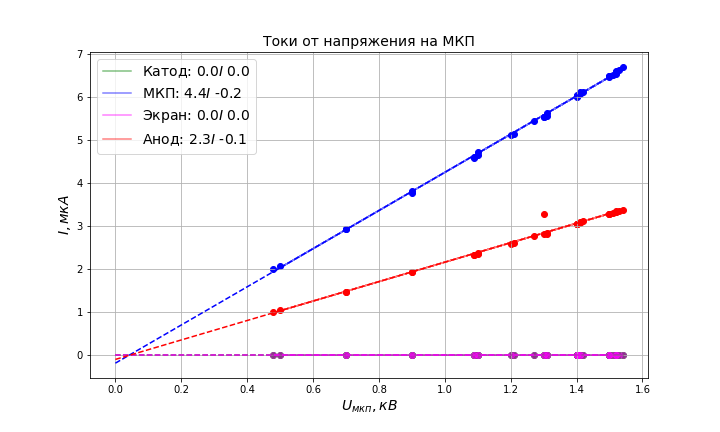
\includegraphics[scale = 0.55]{I_V_MKP.png}
\end{center}

Построим трехмерный график зависимости тока МКП от напряжения на катоде и МКП

\begin{center}
    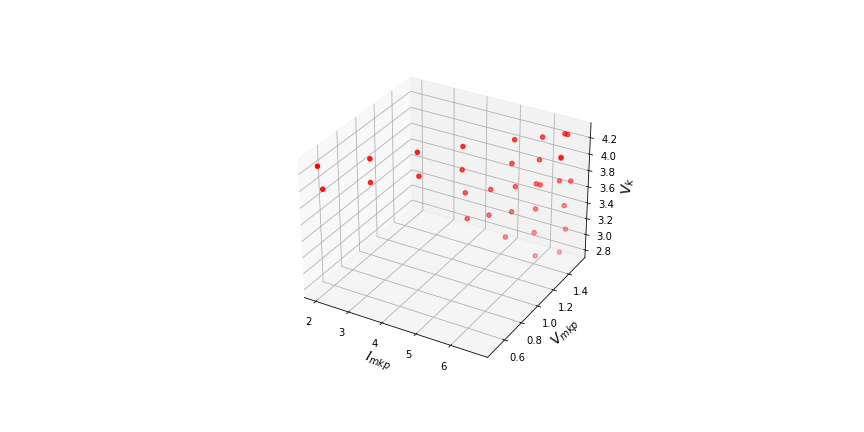
\includegraphics[scale = 0.55]{V_mkp_k_I_mkp.png}
\end{center}


\break

Также построим зависимость токов анода и МКП от напряжения на МКП

\begin{center}
    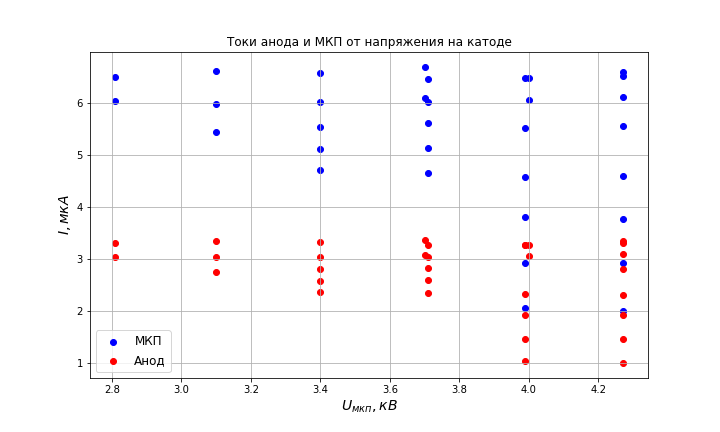
\includegraphics[scale = 0.5]{I_V_K_1.png}
\end{center}

Построим зависимость напряжения на МКП от напряжения на катоде. Получим верхнюю треугольную матрицу. Должны были проварьировать напряжения на катоде и МКП при неизменной яркости изображения, но все перепутали и сделали по-другому

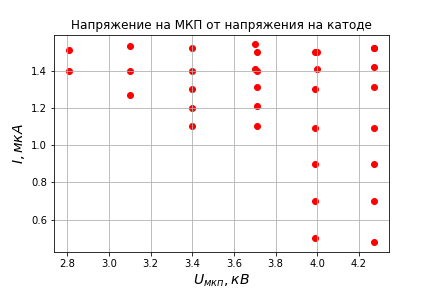
\includegraphics[scale = 0.9]{Triangle.png}

\break

\section{Красивые картиночки}

Установка в цвете(2022г)

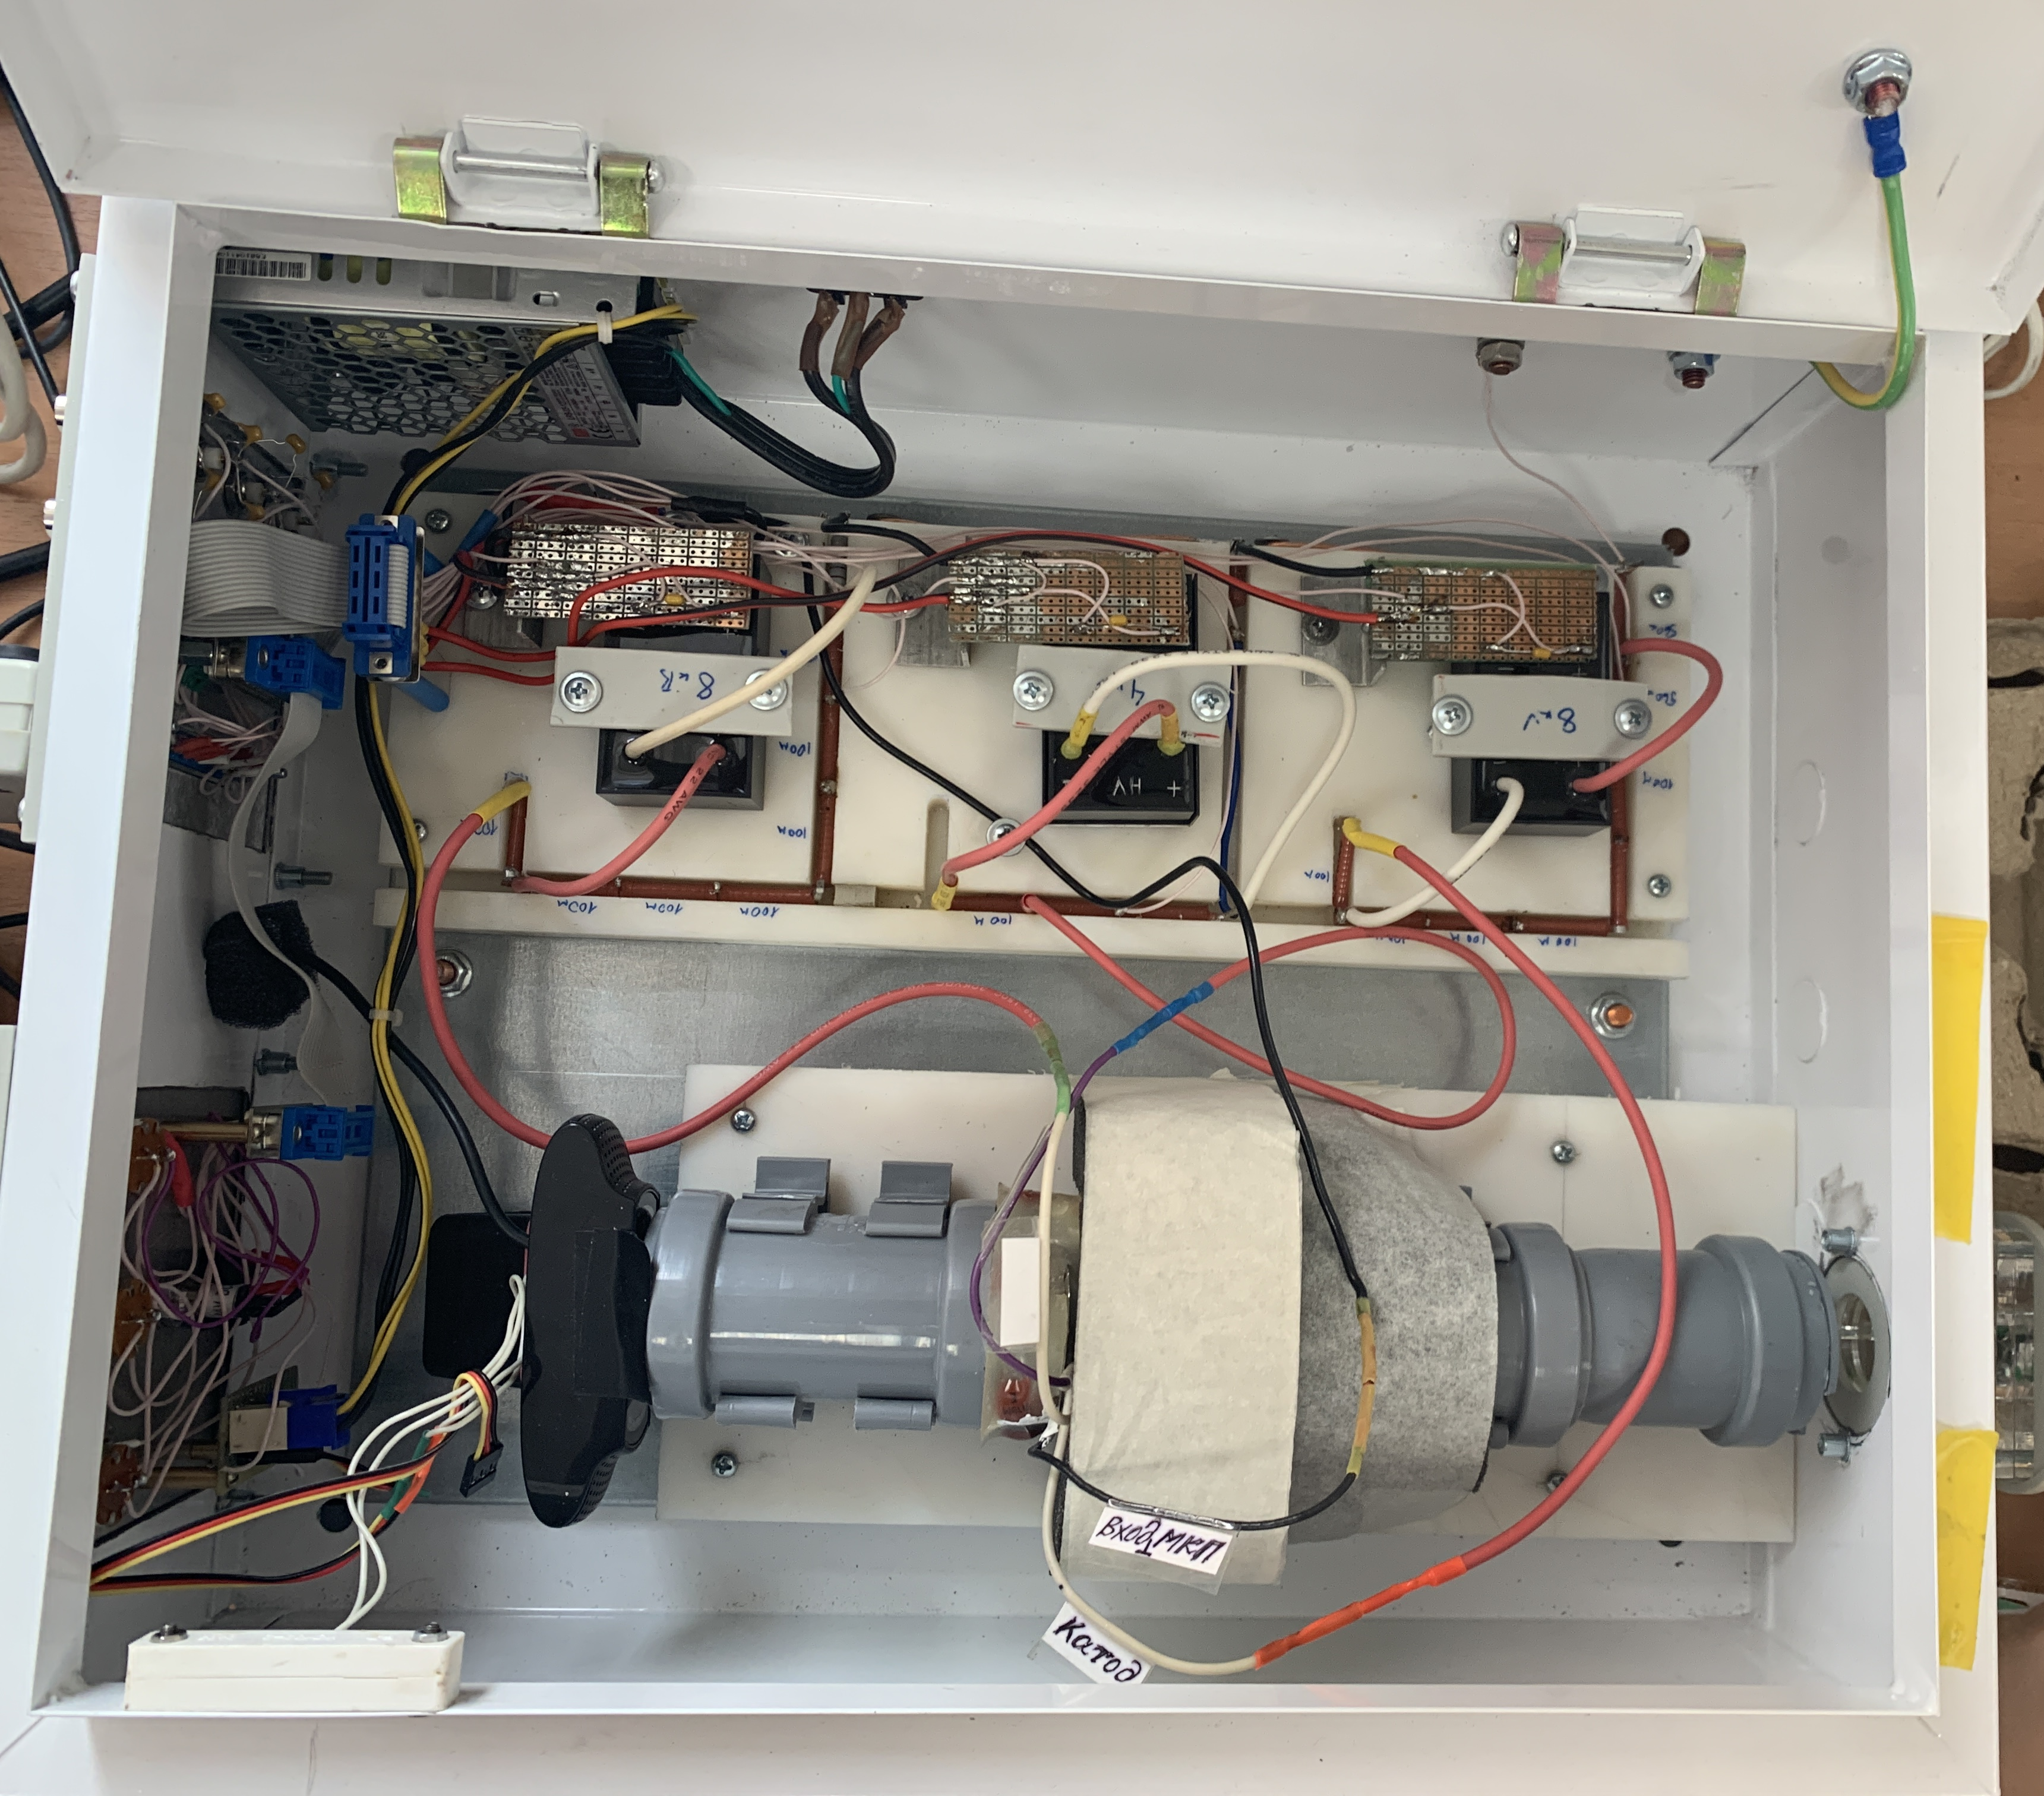
\includegraphics[scale = 0.1]{IMG_3534.jpg}

\hspace

Светофильтры

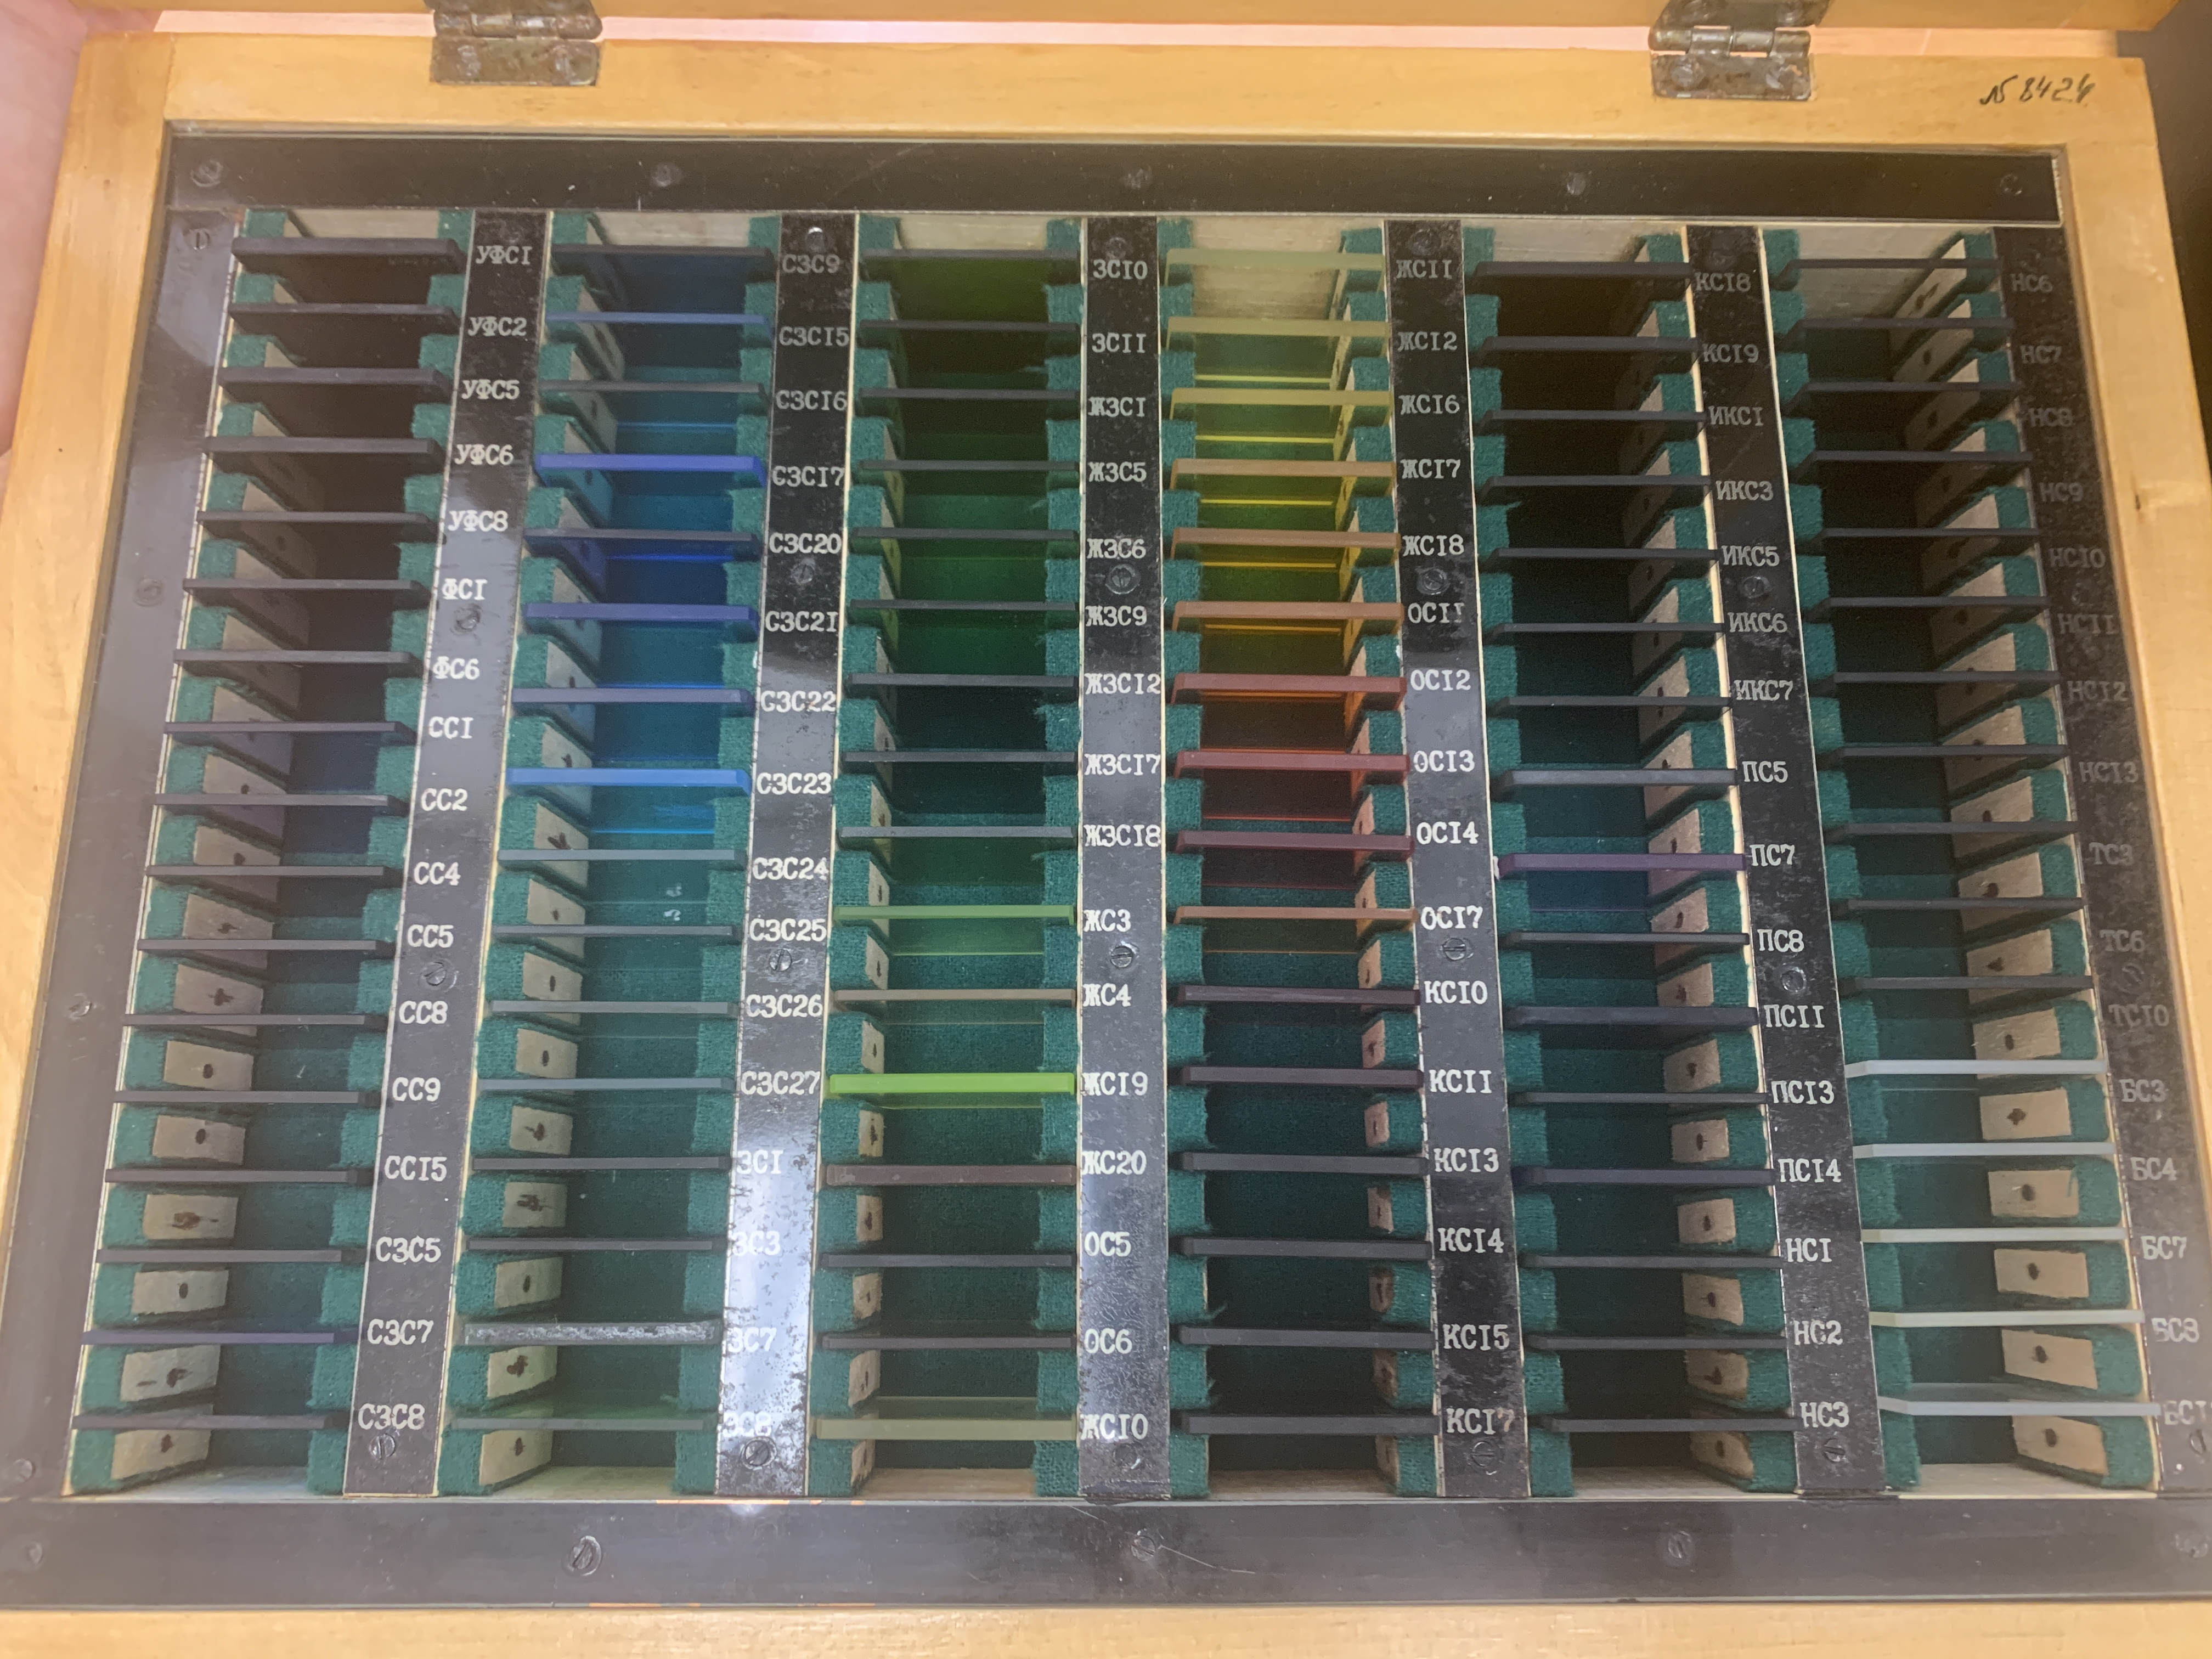
\includegraphics[scale = 0.1]{Пластинки.JPG}

\section{Выводы}


\begin{itemize}
    \item Получили линейную зависимость токов от напряжения на МКП
    \item Получили, что токи не зависят от напряжений на экране и катоде
    \item Наблюдали уменьшение яркости изображения при 
    помещениии светофильтров
    \item Коэффициент усиления не получили, так как не выполнили пункт
    \item Получили верхнюю треугольную матрицу для зависимости напряжения на МКП от напряжения на катоде

\end{itemize}


\begin{tabular}{rrrrrrr}
\toprule
 $V_{mkp}$ & $V_{k}$ & $V_{e}$ & $I_{mkp}$ & $I_{a}$ & $I_{e}$ & $I_k$ \\
\midrule
 1.52 & 4.27 & 3.85 & 6.52 & 3.31 & 0.0 & 0.0 \\
 1.31 & 4.27 & 3.85 & 5.56 & 2.81 & 0.0 & 0.0 \\
 1.09 & 4.27 & 3.85 & 4.60 & 2.31 & 0.0 & 0.0 \\
 0.90 & 4.27 & 3.85 & 3.76 & 1.91 & 0.0 & 0.0 \\
 0.70 & 4.27 & 3.85 & 2.91 & 1.46 & 0.0 & 0.0 \\
 0.48 & 4.27 & 3.85 & 1.99 & 0.99 & 0.0 & 0.0 \\
 1.50 & 3.99 & 3.85 & 6.48 & 3.27 & 0.0 & 0.0 \\
 1.30 & 3.99 & 3.85 & 5.52 & 3.27 & 0.0 & 0.0 \\
 1.09 & 3.99 & 3.85 & 4.58 & 2.32 & 0.0 & 0.0 \\
 0.90 & 3.99 & 3.85 & 3.80 & 1.92 & 0.0 & 0.0 \\
 0.70 & 3.99 & 3.85 & 2.91 & 1.46 & 0.0 & 0.0 \\
 0.50 & 3.99 & 3.85 & 2.06 & 1.03 & 0.0 & 0.0 \\
 1.50 & 3.71 & 3.85 & 6.46 & 3.26 & 0.0 & 0.0 \\
 1.40 & 3.71 & 3.85 & 6.01 & 3.03 & 0.0 & 0.0 \\
 1.31 & 3.71 & 3.85 & 5.61 & 2.83 & 0.0 & 0.0 \\
 1.21 & 3.71 & 3.85 & 5.13 & 2.59 & 0.0 & 0.0 \\
 1.10 & 3.71 & 3.85 & 4.65 & 2.34 & 0.0 & 0.0 \\
 1.52 & 3.40 & 3.85 & 6.58 & 3.32 & 0.0 & 0.0 \\
 1.40 & 3.40 & 3.85 & 6.01 & 3.03 & 0.0 & 0.0 \\
 1.30 & 3.40 & 3.85 & 5.54 & 2.80 & 0.0 & 0.0 \\
 1.20 & 3.40 & 3.85 & 5.11 & 2.58 & 0.0 & 0.0 \\
 1.10 & 3.40 & 3.85 & 4.71 & 2.37 & 0.0 & 0.0 \\
 1.53 & 3.10 & 3.85 & 6.62 & 3.34 & 0.0 & 0.0 \\
 1.40 & 3.10 & 3.85 & 5.99 & 3.03 & 0.0 & 0.0 \\
 1.27 & 3.10 & 3.85 & 5.44 & 2.75 & 0.0 & 0.0 \\
 1.51 & 2.81 & 3.85 & 6.51 & 3.30 & 0.0 & 0.0 \\
 1.40 & 2.81 & 3.85 & 6.04 & 3.04 & 0.0 & 0.0 \\
 1.52 & 4.27 & 3.52 & 6.60 & 3.34 & 0.0 & 0.0 \\
 1.42 & 4.27 & 3.52 & 6.11 & 3.10 & 0.0 & 0.0 \\
 1.50 & 4.00 & 3.52 & 6.48 & 3.27 & 0.0 & 0.0 \\
 1.41 & 4.00 & 3.52 & 6.06 & 3.06 & 0.0 & 0.0 \\
 1.54 & 3.70 & 3.52 & 6.70 & 3.37 & 0.0 & 0.0 \\
 1.41 & 3.70 & 3.52 & 6.10 & 3.08 & 0.0 & 0.0 \\
\bottomrule
\end{tabular}
	
\end{document}
